\documentclass[12pt]{article}
\usepackage[english]{babel}
\usepackage[numbers]{natbib}
\usepackage{graphicx}
\usepackage{xcolor}
\usepackage{sectsty}
\usepackage{float}
\bibliographystyle{apalike}
\setcitestyle{open={[},close={]}}
\sectionfont{\color{DarkBlue}} 
\subsectionfont{\color{LightBlue}}
\subsubsectionfont{\color{LightBlue}}
\paragraphfont{\color{LightBlue}}
\subparagraphfont{\color{LightBlue}}
\definecolor{DarkBlue}{HTML}{4a5a8a}
\definecolor{LightBlue}{HTML}{4f81bf}

\begin{document}
\begin{titlepage}
\begin{flushleft}
\vspace*{1cm}
\Huge
\textbf{Cretaceous Gardens Controller}\\
\vspace{1cm}
\Huge
\textit{Requirements Definition Document}\\
\vspace{1cm}
\Large
\textit{RDD Version 3.0}\\
\vspace{5cm}
\LARGE
Team \#3\\
29 October 2019
\vfill
\Huge
\textbf{CS 460 Software Engineering}
\end{flushleft}
\end{titlepage}
\normalsize
\tableofcontents
\newpage
\section{Introduction}
\paragraph{} The Tyrannosaurus Rex lives among us once again and the opportunity 
to provide an incredible experience has become a reality. The world will be able 
to experience that of which, until now, has only been dreamt. The Cretaceous Gardens
experience will begin the second a visitor steps off the boat and onto the Isla 
Trueno. The visitor will be immersed in Cretaceous Gardens' unique, technological 
advancements: a truly one-of-a-kind luxurious experience. By the time they leave 
they will be already planning their next visit. 

\paragraph{} The purpose of this document is to define the requirements for the 
development of Cretaceous Gardens Controller (CGC) for our billionaire philanthropists 
customers in their new theme park on Isla Trueno near Costa Rica. The CGC is the main 
controller for components like the pay kiosks, cars, and electric fence. The CGC must 
provide sufficient safety, a great user experience, and ought to efficient.

\paragraph{}  Section \ref{obj} outlines the main objectives of the project, 
section \ref{sys} the overall system organization through a high level depiction, 
section \ref{int} outlines interfaces, section \ref{cap} contains the capabilities 
of the system, section \ref{con} provides all known design constraints, and the 
final section provides a reference for potentially unknown terms within the document 
\footnote{Introduction by Anas and Siri.}.  

\section{Objectives}
\label{obj}
\paragraph{} \textit{Four objectives believed to be critical for an 
optimal implementation of a \textit{Cretaceous Gardens Controller} are identified 
here\footnote{Objectives by Anas, Siri and Zeke.}.}
 
	\subsection{Safety}\label{saf}
	\paragraph{} The main objective of the CGC is to provide safe and reliable 
	experiences for the client and its end users. Whether it be electric fences 
	or autonomous vehicles, ensuring safety is of highest priority. The end user
	ought to feel completely safe as should the client whose liability depends on
	this aspect.

	\subsection{Positive User Experience}\label{use}
	\paragraph{} The realization of positive user experiences, in large part, 
	depends on the seamlessness between subsequent interactions with each component
	of a system. For guests, the CGC should be as unimposing as possible in order
	to permit them the fullest immersion offered by Cretaceous Gardens. For the client,
	the system should provide peace of mind that the investment is worthwhile.

	\subsection{Maintainability}\label{mai}
	\paragraph{} The states of the CGC and all \textit{nodes} with which it is to
	communicate should be readily accessible and intelligible. The availability  
	of this information will directly impact the diagnostic and repair speeds 
	anywhere within the system.
	
	\subsection{Efficiency}\label{eff}
	\paragraph{} The CGC is to engender high efficiency and robust functionality. 
	Self-driving cars, pay kiosks, camera system, the global positioning system (GPS), 
	electric fence panels, and all other nodes with which the CGC is to interact 
	must not be burdened by inefficiencies of the CGC. On the contrary, the system
	should be expected to gracefully handle nodal malfunctions, failures, or
	inefficiencies.




\section{Overall System Organization} \label{sys}
\paragraph{} The CGC will be centralized\footnote{System Organization 
by Anas, Santi, Siri, and Zeke.} and will manage all relevant components. Figure 
\ref{fig:blackbox} shows a black box diagram of the CGC. The CGC receives input 
from sensors, user interfaces, and emergency systems like the \textit{Global 
Alarm System} and responds through appropriate output actions as described 
below.

\paragraph{} The Cretaceous Garden Controller will manage self-driving cars whose primary
function will be to transport guests to and from the main exhibit. Pay kiosks, where guests 
are to buy admission tickets, will be locate in the southern region of the island. The admission 
tickets will be in the form of devices called \textit{tokens}, which will grant guests 
access to their assigned vehicles as well.

\paragraph{} The CGC will monitor the position of the T-Rex via GPS and
cameras. In the event of enclosure failure, an emergency mode will be activated;
island-wide alarm sounds will be transmitted, and the autonomous vehicles will
prioritize transporting guests to safety.

\begin{figure}[H]
	\centerline{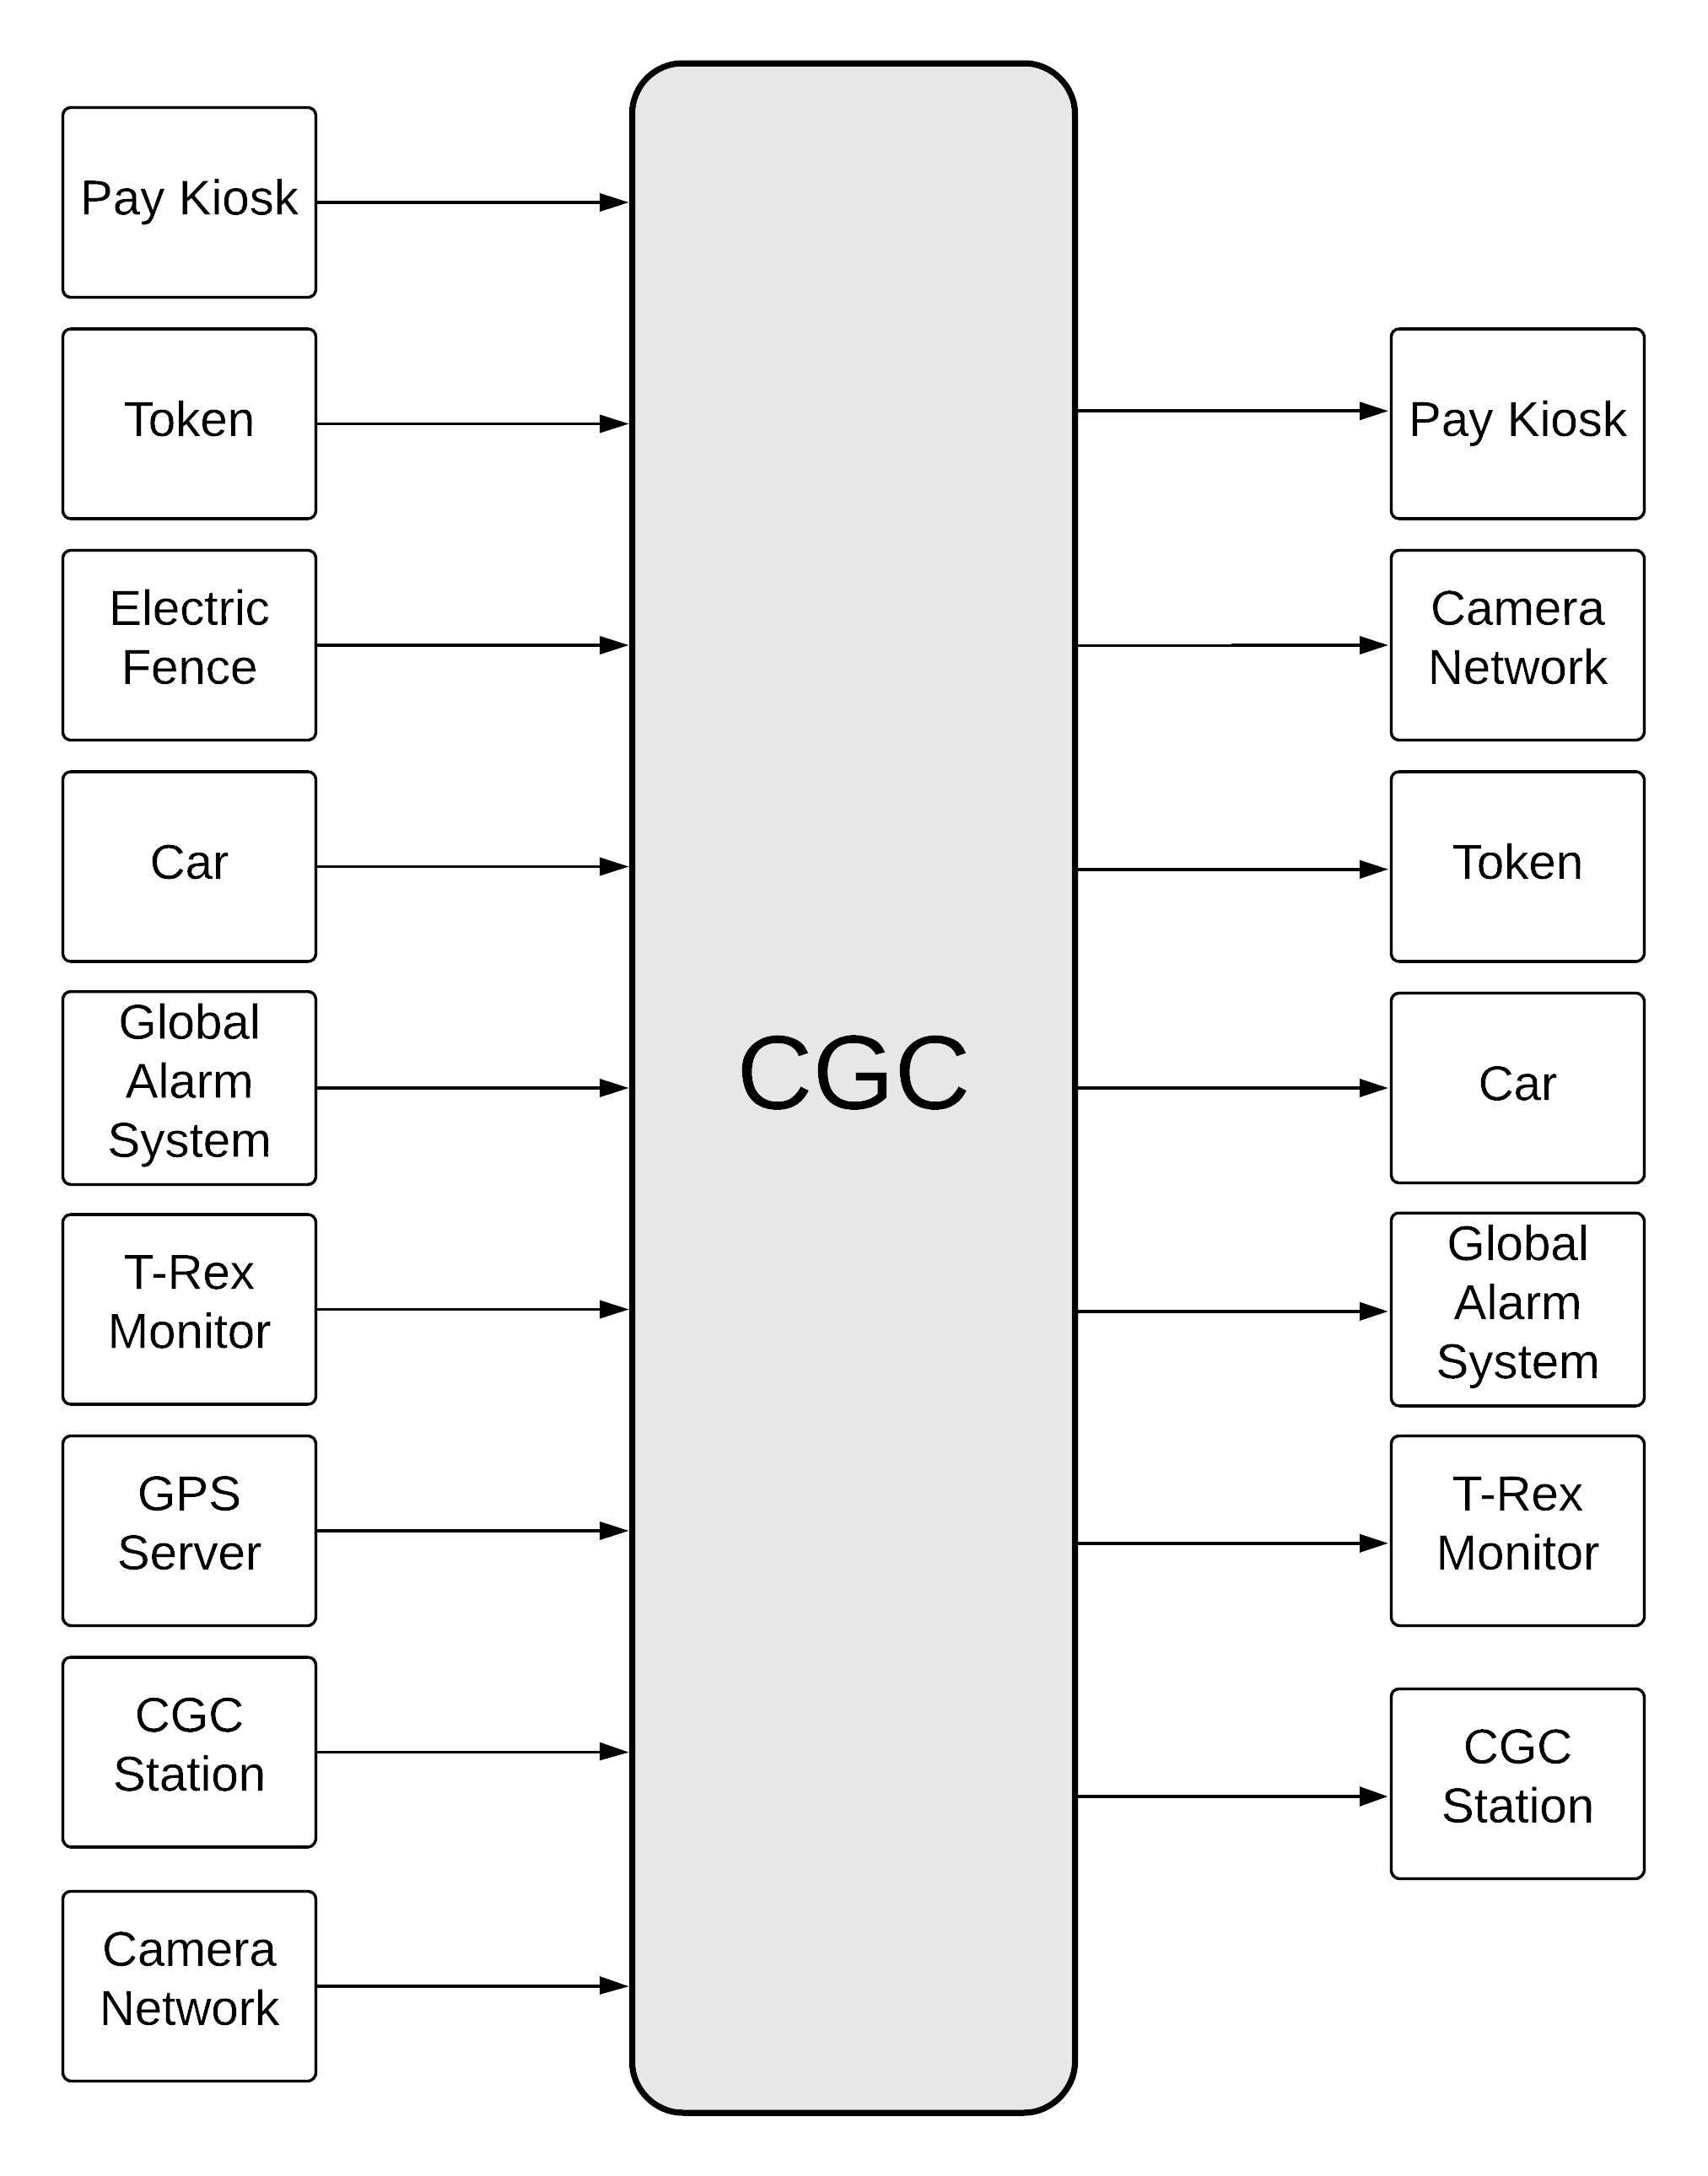
\includegraphics[scale=.15]{CGCBlackBox.png}}
	\caption{A black box of high-level inputs and outputs of the \textit{CGC}.}
	\label{fig:blackbox}
\end{figure}

\section{Interfaces}\label{int}
\paragraph{} \textit{The system interfaces\footnote{Interfaces by Siri, Anas, 
and Zeke} have been grouped into several subsystems. The following list is composed
of devices with which the CGC will interface, and includes the devices' sensors, 
hardware, and features.}

	\subsection{Pay Kiosk}
	\paragraph{} \textit{The purpose of the the Pay Kiosk interface is to connect 
	the physical Pay Kiosks to the CGC, the former of which possesses the following.}
	\paragraph{Sensors}
	\begin{list}{}{}
		\item \textbf{Touch Screen:} senses user interaction. 
		\item \textbf{Credit Card:} accepts all major credit and debit cards. 
		\item \textbf{Cash Receptacle:} accepts cash. 
	\end{list}
		
	\paragraph{Hardware}
	\begin{list}{}{}
		\item \textbf{Change Dispenser:} dispenses change after the purchase of a token.
		\item \textbf{Token Dispenser:} dispenses unique token to guest.
	\end{list}

	\paragraph{Features}
	\begin{list}{}{}
		\item \textbf{Token Builder:} generates unique token from given information (liability waver, name, etc.)
		\item \textbf{Transaction Logger:} provides purchase receipts and stores transactions.
		\item \textbf{Maintenance System:} enables staff to manage issues with the device	
		and maintains device health information. 
	\end{list}

	\subsection{Token}
	\paragraph{} \textit{The Token will act as an interface to multiple systems. 
	It will provide valuable information about the visitor and also interact with 
	the visitor.}
		
	\paragraph{Sensors}
	\begin{list}{}{}
		\item \textbf{Touch Screen:} interacts with the users. 
		\item \textbf{GPS Tracker:} transmits location. 
	\end{list}
		
	\paragraph{Hardware}
	\begin{list}{}{}
		\item \textbf{RFID Chip:} maintains a unique ID and is used for access to 
		multiple systems and areas.
		\item \textbf{Speaker:} transmits alerts and instructions to the guest.
	\end{list}

	\paragraph{Features}
	\begin{list}{}{}
		\item \textbf{Localization:} locatable via GPS.
	\end{list}

	\subsection{Car}
	\paragraph{} \textit{The autonomous car interface is that through which the CGC will
	manage all vehicles, and many of the functions of each vehicle.}
	
	\paragraph{Sensors}
	\begin{list}{}{}
		\item \textbf{RFID Reader:} senses tokens within a defined radius relative 
		to the car, and counts guest tokens within the car.
		\item \textbf{Weight Sensor:} measures weight on each seat, helps determine. 
		\item \textbf{Camera:} used by the car for autonomous driving and also 
		is accessible by CGC.
		\item \textbf{Microphone:} receives guest voice for use in an intercom.
		\item \textbf{GPS Tracker:} transmits location of the car.
	\end{list}
		
	\paragraph{Hardware}
	\begin{list}{}{}
		\item \textbf{Speaker:} transmits alerts, instructions or general audio data.
		\item \textbf{Automatic Door Locks:} engaged upon detection of movement. %% 
		\item \textbf{Wireless Networking:} communicate with the CGC.
	\end{list}
	
	\paragraph{Features}
	\begin{list}{}{}
		\item \textbf{Maintenance System:} enables staff to manage issues with the car 
		and 	maintains car health information.
	\end{list}

	\subsection{T-Rex Monitor}
	\paragraph{} \textit{The T-Rex Monitor interface tracks and monitors the T-Rex. It is 
	critical for employee and visitor safety.}
	\paragraph{Sensors}
	\begin{list}{}{}
		\item \textbf{GPS Tracker:} transmits location of the subject.
		\item \textbf{Heart Rate Sensor:} monitors heart rate (beats per minute) of the T-Rex
		and may be used to gauge stress, hunger, or aggression.
	\end{list}
		
	\paragraph{Hardware}
	\begin{list}{}{}
		\item \textbf{Tranquilizer Injector:} administrates tranquilizer to the subject.
	\end{list}

	\paragraph{Features}
	\begin{list}{}{}
		\item \textbf{Biometrics Monitor:} collects T-Rex biometrics.
		\item \textbf{Maintenance System:} enables staff to manage issues with the device	
		and maintains device health information.
	\end{list}

	\subsection{Camera Network}
	\paragraph{} \textit{The camera network interface communicates with every camera, to 
    all redundant network camera links, and to the digital video recorder (DVR) system 
    that is to record all cameras per retention policy.}		
	
	\paragraph{Sensors}
	\begin{list}{}{}
		\item \textbf{Cameras:} stream video.
	\end{list}
		
	\paragraph{Hardware}
	\begin{list}{}{}
		\item \textbf{DVR:} stores and retains video streams.
		\item \textbf{Hardwired Ethernet:} used for network communication with CGC. 
	\end{list}
	
	\paragraph{Features}
	\begin{list}{}{}
        \item \textbf{Viewing:} ability to view any stream.
        \item \textbf{Maintenance System:} enables staff to manage issues with the device	
		and maintains device health information.
	\end{list}

	\subsection{Electric Fence}
	\paragraph{} \textit{The electric fence interface is that through which the enclosure
	panels are to communicate with the CGC.}
	
	\paragraph{Sensors}
	\begin{list}{}{}
		\item \textbf{Electrical Conduction Sensor:} measures electricity going through 
		electric fence and has the ability to trigger the alarm system in the absence of 
		current. 
	\end{list}
		
	\paragraph{Hardware}
	\begin{list}{}{}
		\item \textbf{Electrical Fence Panels:} electrically conductive enclosure panels.
		\item \textbf{Hardwired Ethernet:} used for network communication with the CGC. 
	\end{list}
	
	\paragraph{Features}
	\begin{list}{}{}
		\item \textbf{Maintenance System:} enables staff to manage issues with the device	and 
		maintains device health information.
	\end{list}

	\subsection{Global Alarm System}
	\paragraph{} \textit{The global alarm system propagates alarm signals throughout the island.}

	\paragraph{Hardware}
	\begin{list}{}{}
		\item \textbf{Speaker:} communicates with a network of public address (PA) speakers.
		\item \textbf{Hardwired Ethernet:} used for network communication with CGC. 
	\end{list}
	
	\paragraph{Features}
	\begin{list}{}{}
		\item \textbf{Maintenance System:} enables staff to manage issues with the device	and 
		maintains device health information.
	\end{list}


	\subsection{CGC Station}
	\paragraph{} \textit{The CGC station interface interacts with staff and features a 
	graphical user interface to analyze and interact with components managed and monitored
	by the CGC.}		
	
	\paragraph{Sensors}
	\begin{list}{}{}
		\item \textbf{Microphone:} receives speech for the intercom and may be used 
		for announcements through the Global Alarm System.
		\item \textbf{Touch Screen:} provides access to the system.
	\end{list}
		
	\paragraph{Hardware}
	\begin{list}{}{}
		\item \textbf{Speaker:} transmits sounds to the station.
		\item \textbf{Hardwired Ethernet:} used for network communication with CGC. 
	\end{list}
	
	\paragraph{Features}
	\begin{list}{}{}
		\item \textbf{Maintenance System:} communicates with all other maintenance systems,
		and may initiate system checks. 
	\end{list}

	\subsection{GPS Server}
	\paragraph{} \textit{The GPS server interface acquires and maintains locations of all 
	active GPS devices (e.g. cars, or tokens)}		
	
	\paragraph{Features}
	\begin{list}{}{}
		\item \textbf{Tracking:} tracks all GPS devices via longitude and latitude coordinates.
        \item \textbf{Services:} third party service to provide GPS services.
	\end{list}

\section{Capabilities}
\label{cap}
\paragraph{}\textit{The capabilities of the system are significantly expansive due to its central role
in the operation of the resort. Thus, the complexity of the system naturally leads to a description
of the broad topography of its capabilities. First is an overview of protocol-related capabilities, then
emergency-supporting capabilities, followed by capabilities that reinforce safety features, and finally an 
overview of its monitoring capabilities.\footnote {Capabilities by Zeke and Matt.}}
	\subsection{Dynamic Protocol Configuration}
	\begin{enumerate}
		\item The CGC will have a set of specified protocols for directing the collection 
		of autonomous vehicles. The protocols will vary among sets of vehicles. For example, 
		a protocol for the visitor vehicles will be executed in the case of an enclosure 
		breach, another for preparation before the arrival of visitors, after their departure 
		(outside business hours), and yet another for scheduled maintenance of the island.
		\item The CGC will enable the configurability of protocols through straightforward 
		interactions with a graphical user interface. This configurability can be thought of
		as functionality for:
		\begin{enumerate}
			\item creation of new protocols.
			\item addition of premade protocols.
			\item removal or extraction of protocols.
			\item modification of existing protocols.
		\end{enumerate}
		\item The CGC will allow for the simulation of any given protocol.
	\end{enumerate}
	
	\subsection{Emergency Features}
	With respect to its emergency mode(s), the CGC will be capable of doing the following:
	\begin{enumerate}
		\item Receive distress or failure signals and propagate responses through the siren and 
		alarm network of the island. 
		\item Communicate with external authorities and emergency personnel.
		\item Be disarmable only through human intervention or complete physical destruction.
		\item The CGC will have the following protocol as a fallback. It should be noted that This can happen 
		any time of day and, for the sake of argument, it will be assumed at that there is peak activity in the garden. 
		In other words, it is assumed that there are \textit{many} visitors at the north end of the island (viewing the T-Rex). 
			\begin{enumerate}
				\item The electric fence interface reports a breach which triggers this \textit{Emergency Protocol}.
				\item The T.Rex monitor interface triggers the device to administer the tranquilizing agent to the subject
				and the subject's heart rate is reported to the CGC every second, as is the subject's location.
				\item Through the Global Alarm System,
					\begin{enumerate}
						\item \textit{All speakers} emit the alarm (protocol-specific) sounds.
						\item Instructions to find and enter the nearest vehicle are propagated through the speakers. 
						\item Instructions are also sent to all active token devices.
						\item Interleaved reassurances that more available vehicles are headed north are also transmitted. 
					\end{enumerate}
				\item{\label{activecars} All \textit{safely occupied} vehicles begin to shuttle people (guests and staff) southward.}
				\item{\label{inactivecars} All \textit{safely inactive} vehicles are dispatched northward.}
				\item{\label{northendcars} Once there, the {safely inactive} vehicles will receive people until \textit{safely occupied}.} 
				\item \ref{activecars}, \ref{inactivecars}, and \ref{northendcars} will be repeated emergency mode is deactivated or until
				all vehicles run out of energy.
			\end{enumerate}
	\end{enumerate}
	
	\subsection{Safety Features} The CGC will possess the following features that 
	serve to fortify safety measures. The CGC will:
	\begin{enumerate}
		\item allow the monitoring of every panel of the enclosure.
		\item allow the monitoring of every camera.
		\item reinforce power backup measures.
		\item maintain redundant uplinks on the network(s).
		\item command a fleet of patrol vehicles around the island.
		\item support a maintenance mode for the real-time repair of any node.
	\end{enumerate}
	
	\subsection{Surveillance and Monitoring Features} With respect to the acquisition of 
	data, the CGC will be able to:
	\begin{enumerate}
		\item track all guests at all times, relative to:
			\begin{enumerate}
				\item others in their groups.
				\item their assigned vehicles.
				\item the whole island.
				\item their current zone within the island.
			\end{enumerate}
		\item track all vehicles at all times.
		\item track the location and biometrics of the T.Rex at all times.
		\item process live video streams of:
		    \begin{enumerate}
		        \item various locations on the island
		        \item the enclosure
		        \item the kiosks
		    \end{enumerate}
		\item perform regular or on-demand audits of the network state.
		\item dynamically account for new nodes or for nodes that are
		taken out for any reason.
	\end{enumerate}
	
	\subsection{Financial Analytics} The CGC will have basic financial functionality as it will
	be able to:
	\begin{enumerate}
		\item provide financial information and basic summary statistics.
		\item identify any striking patterns of cash flow.
		\item maintain long term financial records.
	\end{enumerate}

\section{Design Constraints}
\label{con}
%restrictions placed on the solution space
\paragraph{} \textit{The various constraints \footnote{Constraints by Santi} for the Cretaceous Garden Control are as follows.}
	\subsection{General}
	\begin{itemize}
		\item The Cretaceous Gardens is located on an island.
		\item The Cretaceous Gardens exhibit is dangerous.
		\item The exhibit will be in the northern of the island.
		\item Guests will arrive at the southern end of the island.
		\item Pay Kiosks will be in the southern end of the island.
		\item The T-Rex location must always be known.
		\item Vehicles may accommodate up to 10 guests.
		\item Vehicles must alert guests when their time at the exhibit is up.
		\item Tokens must function as GPS devices.
		\item There must only be one token device per guest.
		\item Live camera streams around the island must be available at all times.
		\item Token devices must be returned upon guest departure.
	\end{itemize}
	
	\subsection{Safety}
	\begin{itemize}
		\item There must be an emergency mode in the event of enclosure failure.
		\item Vehicles must alert and instruct guests in the event of an emergency.
		\item The Alarm System must be audible in the both the northern and southern regions.
		\item Vehicles must facilitate evacuation in the event of an emergency.
		\item There must be a surplus of vehicles at all times on either end of the island.
		\item Tokens must provide additional evacuation information.
		\item Cars must maintain safe speeds at all times.
		\item Cars must lock before moving.
		\item The CGC must communicate to external authorities.
	\end{itemize}

\section{Definition of Terms}
\label{def}
\textit{Here we have some definitions to terms used in the document. This section will help clarify meanings for different 
areas of the document.\footnote {Definition of Terms by Siri and Zeke.}}
\begin{list}{}{}
	\item \textbf{CGC:} Cretaceous Gardens Controller 
	\item \textbf{DVR:} Digital Video Recorder
	\item \textbf{Electrical Conduction:} The movement of electrically charged particles through a transmission medium.
	\item \textbf{GPS:} Global Positioning System 
	\item \textbf{Hardwired Ethernet:} This references the latest IEEE standard for Ethernet utilizing physical cables.
	\item \textbf{Network:} All nodes with which the CGC interacts, the links that connect them to each other and to the
	CGC, the CGC itself, and all related databases.
	\item \textbf{Node:} The generic term that refers to any device connected to the CGC in any way. This includes 
	autonomous vehicles, tokens, the T.Rex monitor, all electric fence panels, all kiosks, and all cameras.
	\item \textbf{Safely Inactive:} A state in which a vehicle is fully functional and ready to be dispatched.
	\item \textbf{Safely Occupied:} A state in which a vehicle contains at least one person, is locked, and is ready to depart.
	\item \textbf{Token:} An interactive device used by the visitor that grants access to locations.
\end{list}

\bibliography{../../ReferenceMaterial/BibTeX/references}
% run latex, then bibtex, then quickbuild all on the tex file
\end{document}
